% LaTeX Template for Project Report, Version 2.0
% (Abstracted from a Major Project Report at CSED, NIT Calicut but can be
% modified easily to use for other reports also.)
%
% Released under Creative Commons Attribution license (CC-BY)
% Info: http://creativecommons.org/licenses/by/3.0/
%
% Created by: Kartik Singhal
% BTech CSE Batch of 2009-13
% NIT Calicut
% Contact Info: kartiksinghal@gmail.com
%
% It is advisable to learn the basics of LaTeX before using this template.
% A good resource to start with is http://en.wikibooks.org/wiki/LaTeX/
%
% All template fields are marked with a pair of angular brackets e.g. <title here>
% except for the ones defining citation names in ref.tex.
%
% Empty space after chapter/section/subsection titles can be used to insert text.
%
% Just compile this file using pdflatex after making all required changes.

\documentclass[12pt,a4paper]{report}
\usepackage[pdftex]{graphicx} %for embedding images
\usepackage{url} %for proper url entries
\usepackage[bookmarks, colorlinks=false, pdfborder={0 0 0}, pdftitle={<pdf title here>}, pdfauthor={<author's name here>}, pdfsubject={<subject here>}, pdfkeywords={<keywords here>}]{hyperref} %for creating links in the pdf version and other additional pdf attributes, no effect on the printed document
%\usepackage[final]{pdfpages} %for embedding another pdf, remove if not required
\usepackage{titlesec}
\usepackage{textcomp}
\usepackage{textgreek}
\usepackage{pdfpages}
\usepackage[toc,page]{appendix}
\usepackage{ragged2e}
\usepackage{amsmath}
\usepackage{amsthm}
\usepackage[margin=1.2 in]{geometry}
\usepackage{longtable}
\titleformat{\chapter}[hang]
  {\normalfont\Huge\bfseries}{\chaptertitlename\thechapter}{1em}{}
\usepackage{graphicx}
\usepackage{amssymb}
\usepackage{epstopdf}
\usepackage{float}

\begin{document}
\renewcommand\bibname{Bibliography} %Renames "Bibliography" to "References" on ref page
\renewcommand{\chaptername}{}
\setcounter{chapter}{0}

%include other pages
\begin{titlepage}

\begin{center}

\textup{\small {\bf October 11th, 2019} \\ MScF}\\[0.2in]

% Title
\Large \textbf {Data Science For Finance \\ Exercise Session 3}\\[0.5in]

       \small \emph{Submitted in partial fulfillment of\\
        the requirements for the course of}
        \vspace{.2in}

       {\bf Data Science for Finance \\ HEC Lausanne \\ University of Lausanne}\\[0.5in]

% Submitted by
\normalsize Submitted by \\
\begin{table}[h]
\centering
\begin{tabular}{lr}\hline \\
Student ID & Names of Students \\ \\ \hline
\\
194 21 437 & Nora Koennyu \\
128 20 858 & Marceau Pierron \\
137 58 495 & David Sasselli \\ 
164 05 136 & Taulant Ukshini \\ \\ \hline 
\end{tabular}
\end{table}

\vspace{.1in}
Under the guidance of\\
{\textbf{Florian Ielpo}}\\[0.2in]

\vfill

% Bottom of the page
%\includegraphics[width=0.18\textwidth]{nitc-logo}\\[0.1in]
%\Large{Department of Computer Science and Engineering}\\
\normalsize
\textsc{University of Lausanne - HEC Lausanne}\\
Unil Internef - 1015 - Lausanne \\
\vspace{0.2cm}
Fall Semester 2019

\end{center}

\end{titlepage}

%\input{certificate}
%\input{abstract}

\pagenumbering{roman} %numbering before main content starts
%\tableofcontents
%\listoftables
%\listoffigures

\newpage
\pagenumbering{arabic} %reset numbering to normal for the main content


\chapter{Exercise 1}

Using 1000 randomly selected sub-periods of 500 days, we analyse the stability of the weights of the optimal portfolio when using different samples to estimate the population parameters.\par \smallskip

Whilst solving this issue, we understand the importance of the number of days of observations needed in order to obtain a stable (i.e. invertible) covariance matrix: a minimum number of observations required to allow us to solve the Markowitz problem without excessively amplifying the magnitude of the optimal weights. \\
An efficient and time-saving method to compute the covariance matrix requires the determination of the eigenvalues and corresponding eigenvectors of the covariance matrix in order to apply a spectral decomposition. Using the spectral theorem implies building two matrices:

\begin{itemize}
    \item The first is a diagonal matrix with eigenvalues on the diagonal and zeros elsewhere.
    \item The second is built combining eigenvectors by column.
\end{itemize}
Note that the inverse of a diagonal matrix $ C $ such as the former is also a diagonal matrix $ D $ with coefficients $ d_{ii} $ on the diagonal such that \(d_{ii}=\frac{1}{c_{ii}}\). \\
When $ c_{ii} $ tends to $ 0 $, $ d_{ii} $ tends to infinity and the stability of any linear transformation resulting from this matrix collapses.
\par\smallskip

When too few observations are used to calculate the covariance matrix, the risk of having very small coefficient on the diagonal grows. The unwanted result reflected on weights instability while applying the Markowitz optimization.
\par\smallskip
In the first series of graphs we’re interested in determining whether the optimal weights variability is due to the sensibility of the estimate of m$\mu$ or $\Sigma$. We define three cases:

\begin{itemize}
\item $\mu$ and $\Sigma$ updated: implying we use the sub-sample of 500 days to compute both: expected log-returns and covariance matrix.
\item $\mu$ updated, sub-sample expected returns and full-sample covariance matrix.
\item $\Sigma$ updated, full-sample expected returns and sub-sample covariance matrix.
\end{itemize}

\newpage
Here we limit our box-plots to the first 20 stocks in order to give the reader a clearer view of the results, it has to be stressed that our calculations and their subsequent results include all 452 stocks from the original data-set.
\par\smallskip
Figure \ref{fig1} demonstrates the stability of the weights for the first 20 stocks of our data-set.\par
The first box-plot shows that the weights are unstable when using the sub-sample of 500 days to determine the optimal allocation by estimating the expected stock returns and volatility.\par
The second shows that using the full-sample to estimate the covariance matrix and the sub-sample to estimate the expected returns results in an apparent stability of the weights regardless of the stock or sub-sample used.\par
The third box-plot shows that using the full-sample to estimate the expected returns and the sub-sample to estimate the covariance provides little to no improvement on the stability of the weights compared to the first case scenario. 

\begin{figure}[H]
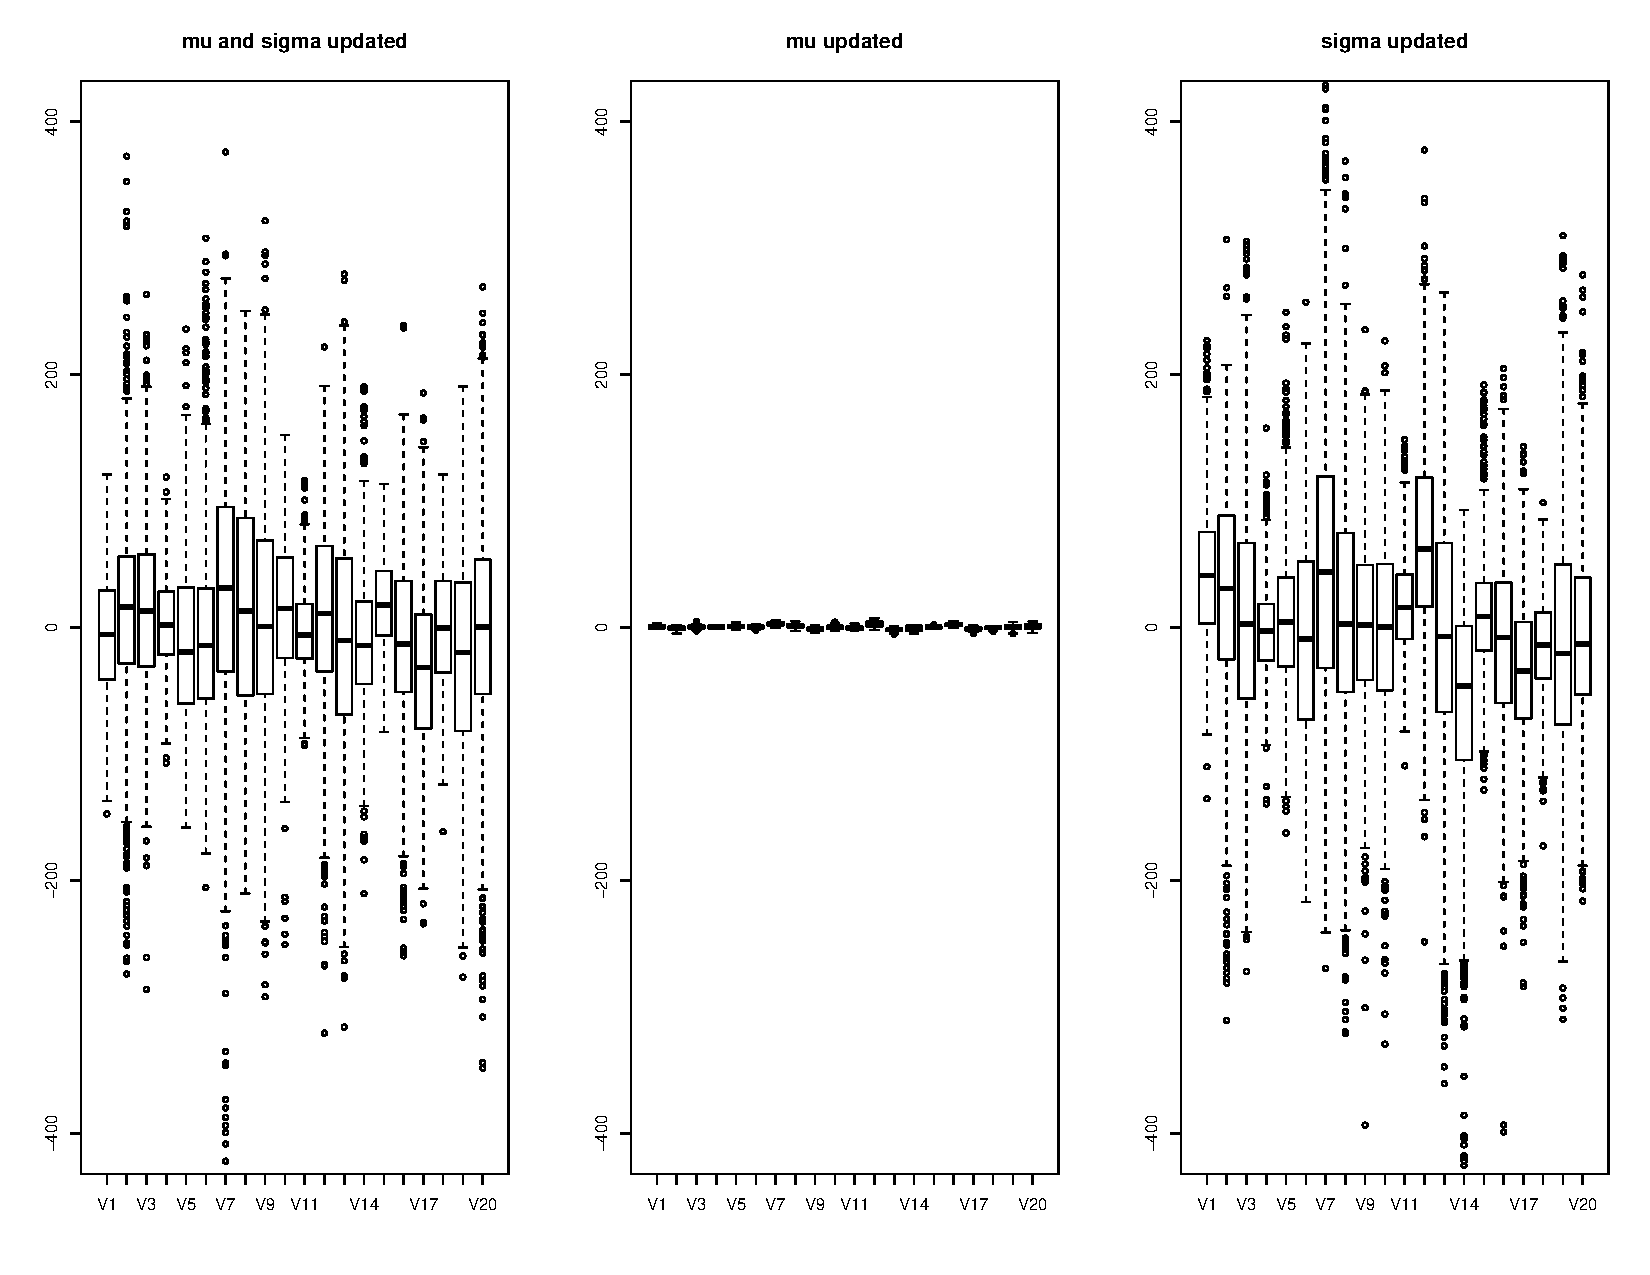
\includegraphics[width=14cm]{Boxplot_question_1.pdf}
\caption{Weight stability for a sub-sample of 500 days}
\label{fig1}
\end{figure}

As a result, we understand that weight instability and variability is primarily due to the estimation of $\Sigma$.
\par\smallskip
We conclude that we need a good estimation of the covariance matrix in order to calculate stable weights for our optimal portfolio. In our example we needed at least a sample size of 500 to get an invertible covariance matrix for 452 stocks, but this sample size is not sufficient to compute stable weights.  
 
 %objective changed to problem definition
\section*{Exercise 2}

We need to show the stability of the weights on the optimal portfolio with shrunk covariance matrices. We use the regularization 
\begin{equation*}
\Sigma_s = \lambda F + (1-\lambda)\Sigma
\end{equation*}
with given $\lambda=0.2$ and with the following two substitutions:
\begin{enumerate}
\item $F=I$, the identity matrix 
\item $F =$ the constant correlation matrix, first used by Ledoit and Wolf. Here we substitute the correlation coefficient between each pair of stocks with the average of the correlation coefficients.  
\end{enumerate} 


In order to compute optimal portfolio weights, the covariance matrix needs to be invertible and needs to be estimated as precisely as possible. 
Shrinkage of the covariance matrix is a way to overcome the problems of its noisy estimation and non-invertibility.
The regularization ensures that the shrunk covariance matrix will be positive definite and thus invertible. We create a convex combination of the estimated covariance matrix, which is potentially positive semi-definite, and a structural matrix $F$, which is designed to be positive definite.

Figure \ref{fig2} compares  
\begin{itemize}
\item our estimates based on the subsample (first boxplot "mu and sigma updated"),
\item our estimates of sigma based on the entire dataset and mu based on the subsample (second boxplot "mu updated"), and
\item the estimates based on the subsample but using the first shrunk covariance matrix, where $F=I$ ("regularized F=I"). 
\end{itemize}

\begin{figure}[H]
%\includegraphics[width=15cm]{DS_Ex3_Q2A.eps}
\caption{Weight stability with shrinkage $F=I$}
\label{fig2}
\end{figure}

Note the different scale on the y-axis. We can see that...

 
Figure \ref{fig3} differs from Figure \ref{fig2} only in the third diagram. Here we compare our previous results with the estimates using the constant correlation matrix.
\begin{figure}[H]
%\includegraphics[width=15cm]{DS_Ex3_Q2B.eps}
\caption{Weight stability with shrinkage using the constant correlation matrix}
\label{fig3}
\end{figure}

We can see that...
 %literature survey included in this
%\chapter{Exercise 3}
%\chapter{Exercise 4}
%\chapter{Exercise 5}
%\cleardoublepage
%\pagebreak
\phantomsection
\addcontentsline{toc}{chapter}{Bibliography}
\begin{thebibliography}{99}

\end{thebibliography}

\begin{appendices}

\chapter{R - Code}

The R-code used to produce the results presented is the following:

\begin{verbatim}

###################################################################
# HEC Lausanne - MScF
# Data Science for Finance
# Exercise Session 2 - 27.09.2019
# Nora Koennyu, Marceau Pierron, Taulant Ukshini, David Sasselli
###################################################################

###################################################################
# Question 1.3 - graphing the distribution of the average randomly
#               drawn from a Poisson distribution with different
#               sample sizes
###################################################################

#initialization
mutotal=c()
parameter=0.5
size=c(30,100,1000,10000)
colours=c("black","red","green","blue")

#sampling
for(i in size){
  mu=c()
  for(j in 1:1000){
    y=rpois(i,parameter)
    s=mean(y)
    mu=c(mu,s)
  }
  
  mutotal=cbind(mutotal,mu)
  
}

#charting the results
postscript("Q1_3plot.eps")
par(bty="n")

plot(density(mutotal[,1]),
     ylim=c(0,50),
     col="black",
     main="",
     xlab="")

for(k in c(2,3,4)){
  lines(density(mutotal[,k]),
        col=colours[k])
}

legend(x="right",y=0.92,c("30 Observations","100 Observations",
                        "1000 Observations","10000 Observations"),
       cex=0.8,
       lty=1,
       col=colours,
       box.lty=0
)
dev.off()

###################################################################
# Question 1.4 - graphing the standard deviation
###################################################################

#calculating standard deviation
mu_func = function(n){
  mu=c()
  for(j in 1:1000){
    x=rpois(n,0.5)
    s=mean(x)
    mu=c(mu,s)
  }
  
  return(sd(mu))
}

func_1 = function(x){
  return(1/sqrt(x))
}

#charting results
postscript("Q1_4plot.eps")
par(bty="n")
plot(func_1,
     main="",
     col="red",
     col.main="black",
     lwd=4,
     xlab="Number of Observations",
     ylab="Volatility of Estimator",
     xlim=c(-50,10000),
     ylim=c(0.01,0.2)
)
i=0

while(i <= 10000){
  points(i,mu_func(i),pch=3)
  i=i+200
}

legend(x="right",y=0.92,c("Estimated Volatility of the Estimator","1/sqrt(n)"),
       cex=0.8,
       lty=c(NA,1),
       col=c("black","red"),
       pch=c(NA,3),
       box.lty=0
)
dev.off()

###################################################################
# Question 1.5 - graphing the distribution of the estimator along
#                with the normal distribution
###################################################################

postscript("Q1_5plot.eps")
layout(matrix(1:4,2,2))
for (i in 1:length(size)){
  temp=(mutotal[,i]-parameter)/(sqrt(parameter))*sqrt(size[i])
  dens=density(temp)
  plot(dens, 
       xlim =c(-4,4),
       ylim =c(0,0.5),
       main=size[i])
  lines(dens$x,dnorm(dens$x),col="red")
}
dev.off()




###################################################################
# Question 2.1 - computing optimal portfolio
###################################################################

#loading data
X=read.delim("data_lausanne_equity.csv",sep=";",header=FALSE)

#calculating optimal weights
X=diff(as.matrix(log(X)),1)
mu2=apply(X,2,mean) 
sigma=cov(X)
sigma_inv=solve(sigma)
gamma=3
w=1/gamma*sigma_inv%*%mu2

###################################################################
#Question 2.2 - computing realized compounded performance
###################################################################


postscript("Q2_2plot.eps")
variance_of_return = t(w)%*%sigma%*%w
performance = t(mu2)%*%w         #expected return on the portfolio               
print(paste("Expected return on the portfolio = ", performance))
print(paste("Expected variance of the portfolio =
        ",variance_of_return))
        
plot(seq(-0.5,0.5,by=0.01), 
     dnorm(seq(-0.5,0.5,by=0.01), mean=performance, sd=sqrt(variance_of_return)),
     xlab="Performance",
     ylab="")
dev.off()


\end{verbatim}

\end{appendices}



\end{document}
